\chapter{Toteutus}
\label{ch:toteutus}
% TODO: Kirjoita uudelleen niin että ei ole yksityiskohtainen.

\section{Yleiskuva}
\label{ch:rcb-sub-yleiskuva}
Kuvassa \ref{fig:rcb-sub-komponenttikaavio} on esitetty komponenttikaavio rcb\_sub-ohjelmasta ja sen käyttämistä kirjastoista. Kuvasta voi nähdä miten eri komponentit ovat relaatiossa keskenään ohjelman kanssa ja mitkä osat kommunikoivat IED-laitteen ja RabbitMQ-palvelimen kanssa.

\begin{figure}[ht!]
	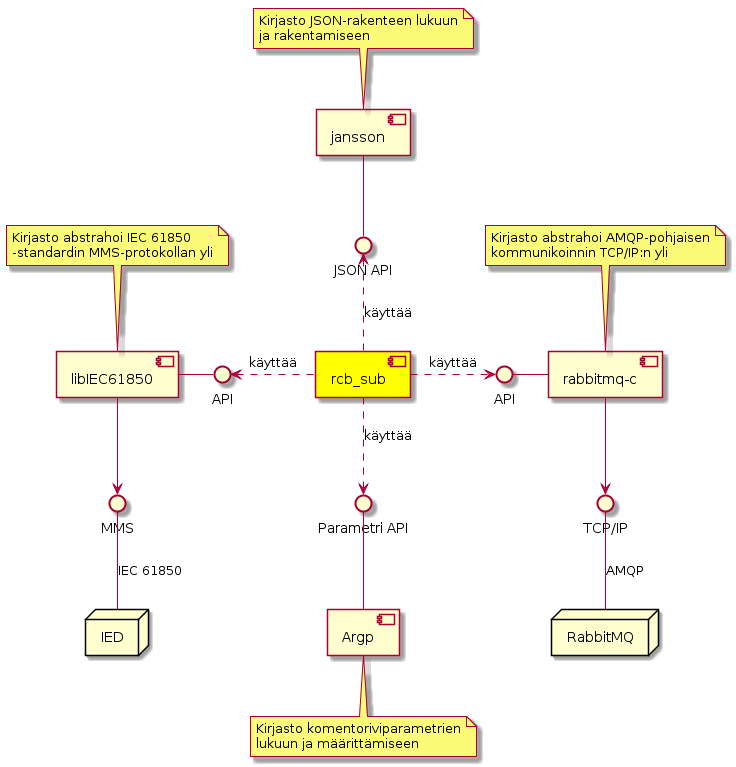
\includegraphics[width=1\textwidth]{pictures/rcb-sub-component-diagram.png}
	\caption{Rcb\_sub-ohjelman komponenttikaavio.}
	\label{fig:rcb-sub-komponenttikaavio}
\end{figure}

Toteutukseen valittiin seuraavat kirjastot:
\begin{itemize}
	\item \emph{libIEC61850} \cite{libIEC61850-repo},
	\item \emph{rabbitmq-c} \cite{rabbitmq-c-repo},
	\item \emph{jansson} \cite{jansson-repo}, ja
	\item \emph{Argp} \cite{argp-glibc-guide}.
\end{itemize}
Kaikki käytetyt kirjastot ovat toteutettu C-kielelle. Kirjastojen tarkoitus on abstrahoida tietyn asian käyttö, ja tarjota käyttäjälle siitä helppokäyttöinen ja ymmärrettävä rajapinta. LibIEC61850-kirjasto abstrahoi IEC 61850 -standardin käyttöä ja hoitaa matalan tason MMS-protokollan kommunikoinnin \cite{libIEC61850-repo}. Samaa kirjastoa käytettiin myös demoversiossa ja kirjaston kerrosarkkitehtuuri esitettiin aikaisemmin kuvassa \ref{fig:libiec61850-layer-architecture}. Kuvassa \ref{fig:rcb-sub-komponenttikaavio} libIEC61850 kommunikoi suoraan IED-laitteen kanssa MMS-protokollaa käyttäen. Rabbitmq-c-kirjasto abstrahoi RabbitMQ-palvelimen käytön ja hoitaa matalan tason AMQP-pohjaisen kommunikoinnin \cite{rabbitmq-c-repo}. Toteutuksessa rabbitmq-c kommunikoi suoraan RabbitMQ-palvelimen kanssa. Jansson-kirjasto abstrahoi JSON-rakenteiden lukua ja käsittelyä C-kielelle \cite{jansson-repo}. Kirjastoa käytettiin muuntamaan IEC 61850 -standardin viesti JSON-muotoon. JSON-rakenne on nähtävissä liitteessä \ref{ch:report-json-format}. Argp-kirjasto auttaa ohjelman komentoriviparametrien määrittämisessä ja käsittelyssä \cite{argp-glibc-guide}. Kirjastolla voidaan toteuttaa \emph{UNIX}-tyyliset \emph{parametrit} (\emph{arguments}) ja \emph{valitsimet/vivut} (\emph{options/switches}). Esimerkki parametreistä on Linux-komento \texttt{mv foo.txt bar.txt}, jossa \emph{foo.txt} ja \emph{bar.txt} ovat parametreja \emph{mv}-ohjelmalle. Vivut voidaan ohjelmalle antaa lyhyessä tai pitkässä muodossa. Esimerkkinä lyhyistä ja pitkistä vivuista \texttt{-b} ja \texttt{-{}-bytes} vastaavasti. Vivut voivat myös vaatia parametreja toimiakseen. Parametri voidaan kirjoittaa lyhyen vivun perään välilyönnillä tai ilman. Pitkän vivun kanssa se erotetaan välilyönnillä tai yhtäsuuruusmerkillä (=). Esimerkkinä lyhyestä \texttt{-w 5} ja pitkästä \texttt{--width=5}, jossa \emph{width}-vivulle annetaan parametrina 5. Kirjasto lisää ohjelmaan automaattisesti Linuxista käyttäjille tutut \texttt{-{}-help} ja \texttt{-{}-version} vivut. Vivulla \texttt{-{}-help} kirjasto tulostaa Linuxilta tutun ohjelman aputekstin käyttäjälle, jossa on esitetty sen kaikki parametrit, vivut ja niiden selitteet \cite{step-by-step-into-argp}.

Kuvassa \ref{fig:rcb-sub-sekvenssikaavio} on esitetty rcb\_sub-ohjelman sekvenssikaavio pääpiirteisestä toiminnasta. Ohjelman suoritus paikoin noudattaa samoja periaatteita kuin demon suoritus (kuvat \ref{fig:sequence-diagram-report-subscription} ja \ref{fig:sequence-diagram-report-subscription-processing}). Seuraavaksi käydään läpi ohjelman pääpiirteinen toiminta ja myöhemmin jokainen kohta tarkemmin läpi kappaleessa \ref{rcb-sub-toiminta}. Ensin ohjelman suoritus alkaa lukemalla annetut parametrit ja vivut Argp-kirjastolla (kohdat 1--2). Parametreissa tulee tiedot yhteyden muodostamiseen IED-laitteelle ja RabbitMQ-palvelimelle (kohdat 3--6). Parametreissa on myös tiedot RCB-instansseista, jotka halutaan IED:ltä tilata. Yhteyksien muodostamisen jälkeen jokainen parametrina annettu RCB käydään läpi silmukassa ja sen arvot ja datajoukon viitteet luetaan IED:ltä (kohdat 7--12). Tämän jälkeen sisäkkäisessä silmukassa luetaan datajoukon viitteiden muuttujien \emph{spesifikaatiot} (kohdat 11--12). Spesifikaatio antaa tiedot attribuuttien pituudesta ja tyypistä, jotka lisätään JSON:iin myöhemmin. Tämän jälkeen tehdään toinen silmukka, jossa jokainen RCB-instanssi tilataan ja niille asetetaan takaisinkutsufunktio (kohdat 13--16). Arvojen kirjoitushetkellä (kohta 15) RCB varataan ja se aloittaa viestien lähettämisen. Jokaisen RCB:n kirjoituksen jälkeen ohjelma jää loputtomaan silmukkaan ottamaan viestejä vastaan (kohdat 17--22). Viestin saapuessa kutsutaan asetettua takaisinkutsufunktiota, jonka parametrina on saapunut viesti (kohta 17). Viesti muutetaan JSON-muotoon jansson-kirjastolla ja julkaistaan RabbitMQ-palvelimelle rabbitmq-c-kirjastolla (kohdat 18--21).

\begin{figure}[ht!]
	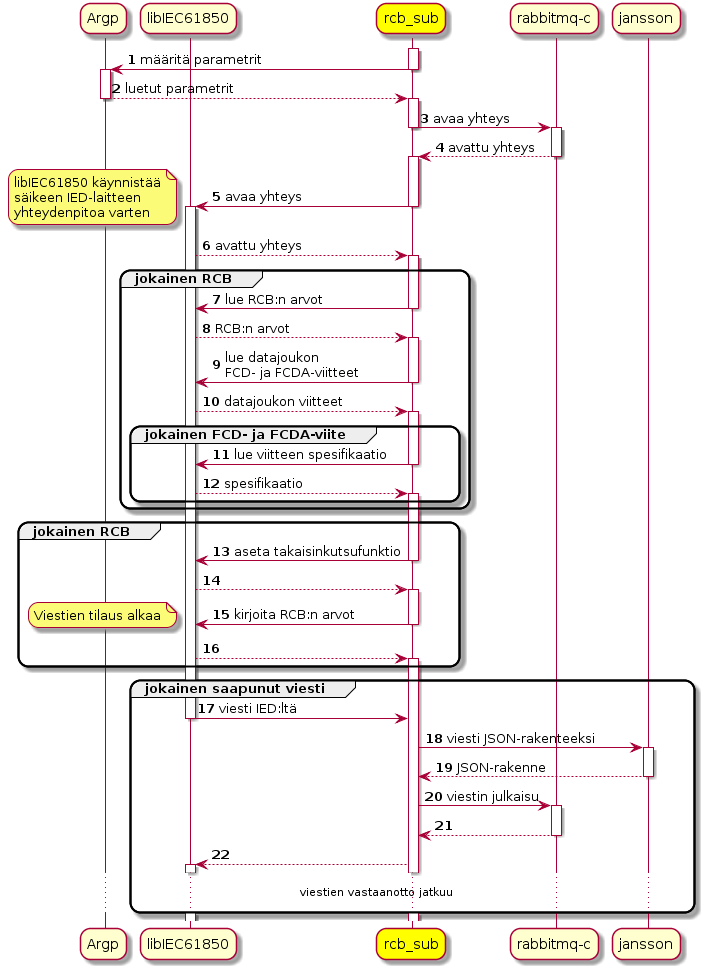
\includegraphics[width=1\textwidth]{pictures/rcb-sub-general-sd.png}
	\caption{Sekvenssikaavio rcb\_sub-ohjelman kokonaistoiminnasta.}
	\label{fig:rcb-sub-sekvenssikaavio}
\end{figure}


\section{Ohjelman toiminta}
\label{rcb-sub-toiminta}
Tulevissa kappaleissa käydään läpi tarkemmin rcb\_sub-ohjelman toimintaa. Kappaleiden järjestys noudattaa kuvassa \ref{fig:rcb-sub-sekvenssikaavio} olevan sekvenssikaavion järjestystä ja jokainen kappale tarkentaa tiettyä osaa siitä. Toisin sanoen ohjelmaa käydään tarkemmin läpi sen suorituksen järjestyksessä.


\subsection{Parametrisointi}
Ohjelma parametrisoitiin Argp-kirjastolla. Kirjasto tarjoaa rajapinnan komentoriviparametrien käsittelyyn ja määrittämiseen. Parametrien muodot ovat tutut muista Linux-käyt\-tö\-jär\-jes\-tel\-män parametreista ja samaa periaatetta käytettiin tässäkin ohjelmassa. Kirjasto myös lisäsi ohjelmaan automaattisesti aputekstin käyttäjää varten. Aputeksti sisältää tietoa ohjelman parametreista ja niiden käytöstä. Aputekstin pystyi tulostamaan vivulla \texttt{-{}-help}. Liitteessä \ref{ch:rcb-sub-help-output} on esitetty ohjelman tulostama aputeksti. Liitteestä voi myös nähdä kaikki ohjelman parametrit ja lyhyen selityksen mihin kutakin käytetään. Aputeksti ei sinänsä ollut tarpeellinen, koska muu järjestelmä hallitsee ohjelman suoritusta ja parametrien antamista. Se kuitenkin päätettiin lisätä pienen vaivan vuoksi ja toimii hyvänä dokumentaationa myöhemmin.

Ohjelmiston parametrien ja vipujen voidaan ajatella koostuvan kolmesta eri ryhmästä (liite \ref{ch:rcb-sub-help-output} rivit 1--4). Ensin päätason vaihtoehtoiset vivut \texttt{OPTIONS} (rivi 1). Pakolliset parametrit \texttt{EXCHANGE} ja \texttt{ROUTING\_KEY} (rivi 2). Viimeisenä ryhmänä \texttt{RCB\_REF} parametri ja siihen liittyvät vivut \texttt{RCB\_OPTIONS} (rivi 3). Näitä ryhmiä voi olla n-kappaletta, mutta vähintään yksi. Liitteessä \ref{ch:rcb-sub-help-output} riveillä 71--72 on esitetty esimerkki, joka tilaa viestit IED-laitteelta osoitteesta 192.168.2.220. AMQP-vaihteen nimi on \emph{testexchange} ja reititysavaimen nimi on \emph{testkey}. IED-laitteelta tilataan RCB-instanssi viitteellä MY\_LD0""/""LLN0"".""BR"".""rcbMeas01. Instanssille asetetaan yleinen kysely (\texttt{-g1}), liipaisimet (\texttt{-t27}) ja viestin vaihtoehtoiset kentät (\texttt{-o16}). Liipaisimet ja vaihtoehtoiset kentät annetaan numeroarvoilla summaamalla niitä yhteen. Vaihtoehdot näkee ohjelman aputekstistä (esimerkiksi liipaisimet riveillä 53--58).

Suurin osa \texttt{OPTION} vivuista ovat itsestäänselviä. Esimerkkinä \texttt{-{}-amqp-host}, joka kertoo AMQP-pal\-ve\-li\-men IP-osoitteen, ja \texttt{-{}-ied-host}, joka kertoo IED-laitteen IP-osoitteen. Parametrit \texttt{EXCHANGE} ja \texttt{ROUTING\_KEY} määrittävät nimet RabbitMQ-pal\-ve\-li\-men vaihteelle ja reititysavaimelle. Parametri \texttt{RCB\_REF} määrittää viitteen tilattavaan RCB-instanssiin IED-laitteella. Tätä seuraa vaihtoehtoinen \texttt{RCB\_OPTIONS} vipu, joka määrittää edeltävän instanssin kirjoitettavat arvot ennen tilausta. Sillä voidaan määrittää käytetyt vaihtoehtoiset kentät (\texttt{-{}-opt-fields}), käytetyt liipaisimet (\texttt{-{}-trigger}) ja pyydetäänkö yleistä kyselyä ennen muita viestejä (\texttt{-{}-gi}). Liipaisimien nimet vastaavat aikaisemmin kappaleessa \ref{ch:rcb-toiminta} esitettyjä arvoja ja numeeriset arvot tulevat libIEC61850-kirjastosta. Vaihtoehtoisten kenttien nimet vastaavat aikaisemmin taulukossa \ref{tab:iec61850-optional-fields-definition} esitettyjä arvoja ja sen numeeriset arvot tulevat myös libIEC61850-kirjastosta.

\subsection{Yhteyksien muodostus}
Parametrien luvun jälkeen ohjelma muodostaa yhteydet ensin RabbitMQ-palvelimelle ja sen jälkeen IED-laitteelle. Kuvassa \ref{fig:rcb-sub-open-connections} on esitetty sekvenssikaavio, joka näyttää mitä kirjaston funktioita ohjelma kutsuu missäkin järjestyksessä. Funktiot ja niiden parametrit voi tarkemmin tarkistaa kirjastojen omista dokumentaatioista \cite{libIEC61850-doc} \cite{rabbitmq-c-repo}. Tämä tarkentaa yleiskuvasta \ref{fig:rcb-sub-sekvenssikaavio} kohdat 3--6. Kaaviossa ohjelma muodostaa yhteydet vain kerran. Ohjelma on kuitenkin toteutettu niin, että se yrittää muodostaa yhteydet uudestaan vikatilanteissa. Jos muodostus ei onnistu, ohjelma kirjoittaa lokin tapahtuneesta ja odottaa hetken ennen uudelleen yritystä.

\begin{figure}[ht!]
	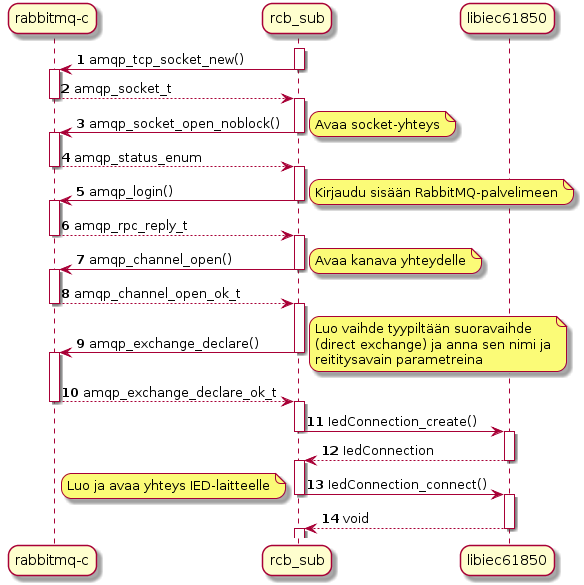
\includegraphics[width=1\textwidth]{pictures/rcb-sub-open-connections.png}
	\caption{Sekvenssikaavio kuinka rcb\_sub avaa yhteydet RabbitMQ-palvelimelle ja IED-laitteelle.}
	\label{fig:rcb-sub-open-connections}
\end{figure}

Yhteyden avauksen ja sisäänkirjautumisen jälkeen ohjelma avaa kanavan kohdassa 7--8. Kanava on yhteyden päälle avattu oma erillinen kommunikointiväylä, joka ei sotkeudu muihin kanaviin. Yhteen avattuun yhteyteen voi olla avattuna monta eri kanavaa. Kanavat mahdollistavat sen, että sama yhteys voidaan jakaa monen säikeen kanssa. Kohdassa 9 kutsutaan funktiota \texttt{amqp\_exchange\_declare()}. Funktio määrittää vaihteen tyyppiä suoravaihde RabbitMQ-palvelimelle. Suoravaihde on AMQP-vaihteen tyyppi, joka määrittää kuinka viestejä reititetään reititysavaimen perusteella. Vaihteen ja sen tyyppien toimintaperiaatteet voi lukea AMQP:n dokumentaatiosta \cite[s.~26--28]{AMQP-specification}.


\subsection{IED:n attribuuttien tyyppin ja koon luku}
Yhteyksien muodostamisen jälkeen ohjelma käy läpi silmukassa jokaisen parametrina annetun RCB:n viitteen. Lukee RCB:n datajoukon viitteet ja selvittää jokaisen viitatun attribuutin spesifikaatiot, eli sen oikean viitteen, tyypin ja koon. Kuvassa \ref{fig:rcb-sub-reading-specifications} on esitetty sekvenssikaavio toiminnasta. Kuva tarkentaa yleiskuvassa \ref{fig:rcb-sub-sekvenssikaavio} kohtia 7--12.

\begin{figure}[ht!]
	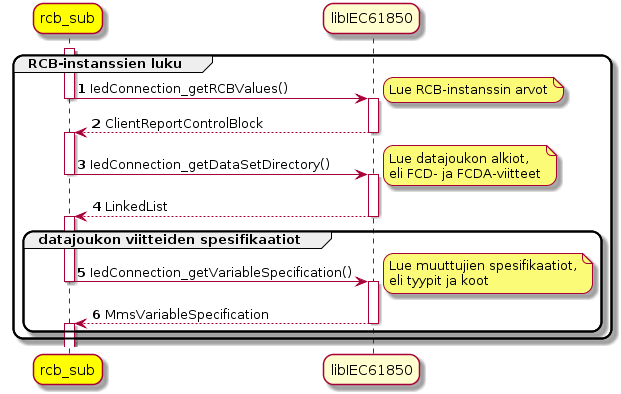
\includegraphics[width=1\textwidth]{pictures/rcb-sub-reading-specifications.png}
	\caption{Sekvenssikaavio kuinka rcb\_sub lukee RCB-instanssin arvot ja muuttujien spesifikaatiot.}
	\label{fig:rcb-sub-reading-specifications}
\end{figure}

Ensin RCB:sta luetaan sen tiedot IED-laitteelta (kohdat 1--2). RCB:ltä saadaan tieto mihin datajoukkoon se on liitetty. Tätä käsiteltiin kappaleessa \ref{ch:rcb-toiminta} ja taulukossa \ref{tab:iec61850-brcb-class-definition} kenttä \emph{DatSet}, joka kertoo käytetyn datajoukon viitteen. Tällä tiedolla ohjelma voi lukea datajoukon FCD- ja FCDA-viitteet (kohdat 3--4). Tästä saadaan jokainen viite listassa, joka käydään läpi silmukassa kohdissa 5--6. Jokaiselle viitteelle luetaan sen spesifikaatio. Spesifikaatiorakenne sisältää sisäkkäisiä spesifikaatioita, jos viite viittaa moneen muuttujaan IED-laitteen hierarkiassa. Tämä tapahtuu samalla periaatteella, jolla FCD- ja FCDA-viitteet viittaavat moneen muuttujaan hierarkiassa alaspäin. Jokainen luettu viite tallennetaan ja niitä käytetään myöhemmin viestin kanssa JSON-rakenteessa. Esimerkkinä liitteessä \ref{ch:report-json-format} riveillä 21--22 tyyppi ja koko -tiedot.


\subsection{Viestien tilaus}
Ohjelman luettua kaikki muuttujien spesifikaatiot. Ohjelma tilaa silmukassa parametrina annetut RCB-instanssit. Kuvassa \ref{fig:rcb-sub-subscribe-reports} on esitetty sekvenssikaavio toiminnasta. Kuva tarkentaa yleiskuvassa \ref{fig:rcb-sub-sekvenssikaavio} kohtia 13--16.

\begin{figure}[ht!]
	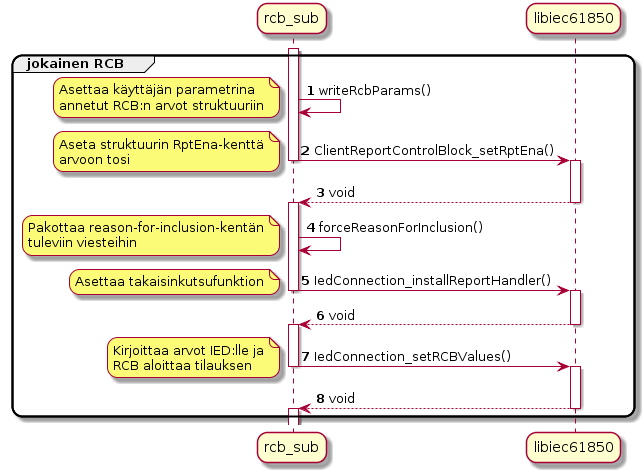
\includegraphics[width=1\textwidth]{pictures/rcb-sub-subscribe-reports.png}
	\caption{Sekvenssikaavio kuinka rcb\_sub tilaa RCB-instanssit.}
	\label{fig:rcb-sub-subscribe-reports}
\end{figure}

Ohjelma käsittelee libIEC61850-kirjaston tarjoamaa \emph{ClientReportControlBlock}-struk\-tuu\-rin instanssia. Kirjasto palauttaa struktuurin instanssin, kun RCB:n arvot luetaan IED-laitteelta. Kaikki RCB:lle kirjoitettavat arvot asetetaan instanssiin ennen IED-laitteelle kirjoitusta. Näitä arvoja ovat ohjelmalle parametreinä annetut arvot, kuten liipaisimet ja vaihtoehtoiset kentät. Tämän ohjelma tekee kutsumalla omaa funktiota \texttt{write""Rcb""Params()} (kohta 1). Tämän jälkeen ohjelma asettaa RCB:n \emph{RptEna}-kentän arvoksi tosi (kohdat 2--3). Tämä kenttä kontrolloi RCB-instanssin varausta ja onko tilaus päällä. Seuraavaksi ohjelma pakottaa viestiin vaihtoehtoisen kentän \emph{reason-for-inclusion} (kohta 4). Tätä kenttää tarvitaan, jotta aikaisemmin luetut spesifikaatiotiedot saadaan yhdistettyä saapuneeseen viestiin. Tämän jälkeen asetetaan takaisinkutsufunktio, jota kirjasto kutsuu kun viesti saapuu (kohdat 5--6). Viimeisenä struktuurin arvot kirjoitetaan IED:llä olevalle RCB:lle (kohdat 7--8). Tämä varaa RCB-instanssin kirjoittavalle asiakkaalle, ja aloittaa tilauksen, jos RptEna-kentän arvo oli tosi. RCB tulee lähettämään viestejä ohjelmalle samalla kun silmukan muilla kierroksilla käsitellään tilaamattomia RCB-instansseja.


\subsection{JSON:in muodostaminen ja julkaisu}
Viestin saapuessa libIEC61580-kirjasto kutsuu asetettua takaisinkutsufunktiota. Takaisinkutsufunktio muuttaa viestin JSON-muotoon ja lisäsi siihen aikaisemmin luetut muuttujien oikeat viitteet, tyypit ja koot. Tämän jälkeen JSON-julkaistiin RabbitMQ-palvelimelle. Kuvissa \ref{fig:rcb-sub-report-to-json-1} ja \ref{fig:rcb-sub-report-to-json-2} on esitetty sekvenssikaaviolla, kuinka ohjelma muuttaa viestin JSON:iksi ja julkaisee RabbitMQ:lle. Kuva \ref{fig:rcb-sub-report-to-json-1} jatkuu kuvassa \ref{fig:rcb-sub-report-to-json-2}. Kuva \ref{fig:rcb-sub-report-to-json-1} tarkentaa yleiskuvan \ref{fig:rcb-sub-sekvenssikaavio} kohtia 17--19 ja kuva \ref{fig:rcb-sub-report-to-json-2} kohtia 20--22. Aikaisemmin mainittiin, että libIEC61850-kirjasto toteuttaa sisäisen puskurin viestien vastaanottoon ja käsittelee siitä yhden viestin kerrallaan. Kirjasto varaa yhden puskurin yhteyttä kohti. Puskurista käsitellään seuraava viesti, kun edellinen takaisinkutsufunktion suoritus on palannut. Rcb\_sub avaa vain yhden yhteyden IED-laitteeseen. Seurauksena on, että viestejä ei prosessoida rinnakkain missään vaiheessa suoritusta.

\begin{figure}[ht!]
	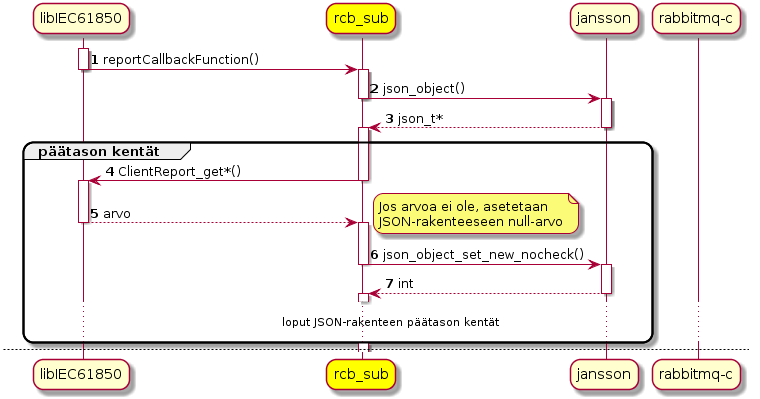
\includegraphics[width=1\textwidth]{pictures/rcb-sub-report-to-json.png}
	\caption{Sekvenssikaavio kuinka rcb\_sub muodostaa JSON:nin päätason kentät.}
	\label{fig:rcb-sub-report-to-json-1}
\end{figure}

Kuvassa \ref{fig:rcb-sub-report-to-json-1} suoritus alkaa, kun libIEC61850-kirjasto kutsuu takaisinkutsufunktiota. Funktiolle annetaan parametrina saapunut viesti \emph{ClientReport}-struktuurin instanssina (kohta 1). Tämän jälkeen ohjelma käy läpi viestin jokaisen päätason kentän ja lisää ne JSON-rakenteeseen. Osa viestin kentistä on vaihtoehtoisia riippuen siitä, mitä käyttäjä asetti \texttt{-{}-opt-fields} vivun parametrilla. Jos arvoa viestissä ei ole, korvataan se null-arvolla JSON:iin. Tämän jälkeen suoritus jatkuu kuvasta \ref{fig:rcb-sub-report-to-json-1} kuvaan \ref{fig:rcb-sub-report-to-json-2}.

\begin{figure}[ht!]
	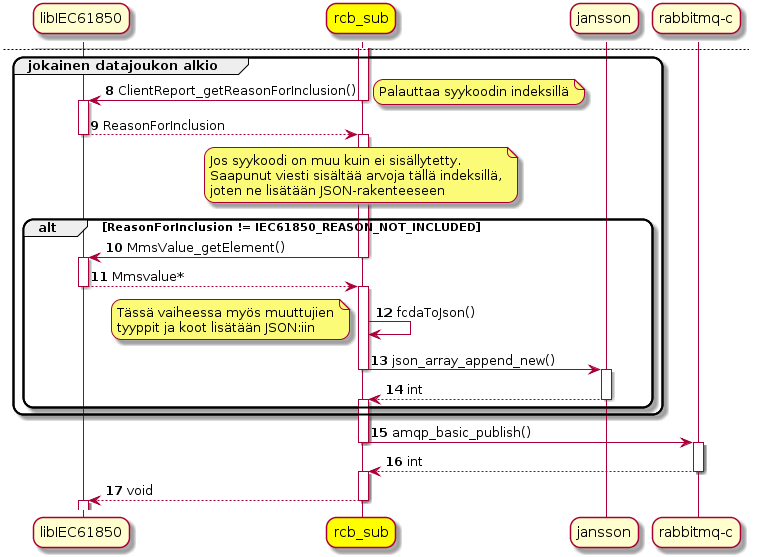
\includegraphics[width=1\textwidth]{pictures/rcb-sub-report-to-json_001.png}
	\caption{Sekvenssikaavio kuinka rcb\_sub lisää JSON:iin muuttujat viestistä.}
	\label{fig:rcb-sub-report-to-json-2}
\end{figure}

Päätason viestin kenttien jälkeen ohjelma käy läpi silmukassa viestin datajoukon indeksit (kuvassa \ref{fig:rcb-sub-report-to-json-2} kohdat 8--14). Viesti sisältää vain ne datajoukon alkiot, jotka sisältyivät viestiin. Ongelmana on, että viesti ei sisällä indeksiä tai tietoa siitä mikä datajoukon alkio on kyseessä. Tämän tiedon saamiseksi ohjelman pakottaa syykoodin päälle viestiin. Tämän avulla datajoukon indeksiltä voidaan kysyä syykoodia (kohdat 8--9). Jos datajoukon alkio ei ole viestissä, kirjaston funktio \texttt{Client""Report""\_""get""Reason""For""Inclusion()} palauttaa arvon \texttt{IEC61850""\_""REASON""\_""NOT""\_""INCLUDED}. Tämän avulla löydetään datajoukon viitteistä indeksi, joka sisällytettiin viestiin. Indeksin ollessa viestissä suoritetaan kohdat 10--14, muuten mennään seuraavaan indeksiin ja toistetaan kohdat 8--9. Datajoukon indeksi tarvitaan, jotta aiemmin luetut spesifikaatiot saadaan yhdistettyä attribuutteihin arvojen kanssa. Datajoukon indeksillä, viestin arvoilla ja muuttujien tyypeillä ja koolla saadaan rakennettua loppuosa JSON-rakenteesta. Kuvassa \ref{fig:rcb-sub-report-to-json-2} oleva silmukka rakentaa liitteessä \ref{ch:report-json-format} olevan values-taulun alkaen riviltä 7. JSON:in sisempi values-taulu (rivi 13) on lista FCD- tai FCDA-viitteen muuttujia, mitä se viittaa arvoineen. Tämä taulukko muodostetaan kuvan \ref{fig:rcb-sub-report-to-json-2} kohdassa 12 funktiolla \texttt{fcdaToJson()} ja lisätään JSON:iin kohdassa 13. Lopuksi viesti lähetetään RabbitMQ-palvelimelle funktiolla \texttt{amqp\_basic\_publish()} ja takaisinkutsufunktio palaa (kohdat 15--17).